\documentclass[12pt]{article}
\usepackage[T1]{fontenc}
\usepackage[utf8]{inputenc}
\usepackage[table]{xcolor}
\usepackage{hyperref}
\usepackage{mathtools}
\usepackage{graphicx} 
\usepackage{titlesec}
\usepackage{float}
\usepackage{tabularx,booktabs,caption,ragged2e}
\usepackage[style=verbose]{biblatex}
\usepackage{eurosym}
\usepackage{amsmath , amsfonts, amssymb}
\usepackage{adjustbox}
\usepackage{fancyhdr}
\usepackage{multicol}
\addbibresource{bibliographie.bib}
\setlength{\parindent}{0pt}
\setlength{\headheight}{14.61858pt}
\captionsetup{skip=0.333\baselineskip}
\usepackage{geometry}
\geometry{a4paper,textwidth=480pt}

\setlength{\tabcolsep}{12pt}
%\titleformat{\section}{format}


\begin{document}
\begin{titlepage}
    \centering
    
\includegraphics[width=0.25\textwidth]{um.png}\par\vspace{0.5cm}
    {\Large Université de Montpellier \par}
    {\large Faculté d'économie\par}
    \vfill
    {\huge\bfseries Analyse Financière\par}
    \vspace{0.1cm}
    {\Large Groupe TotalEnergies\par}
    \vspace{0.5cm}
    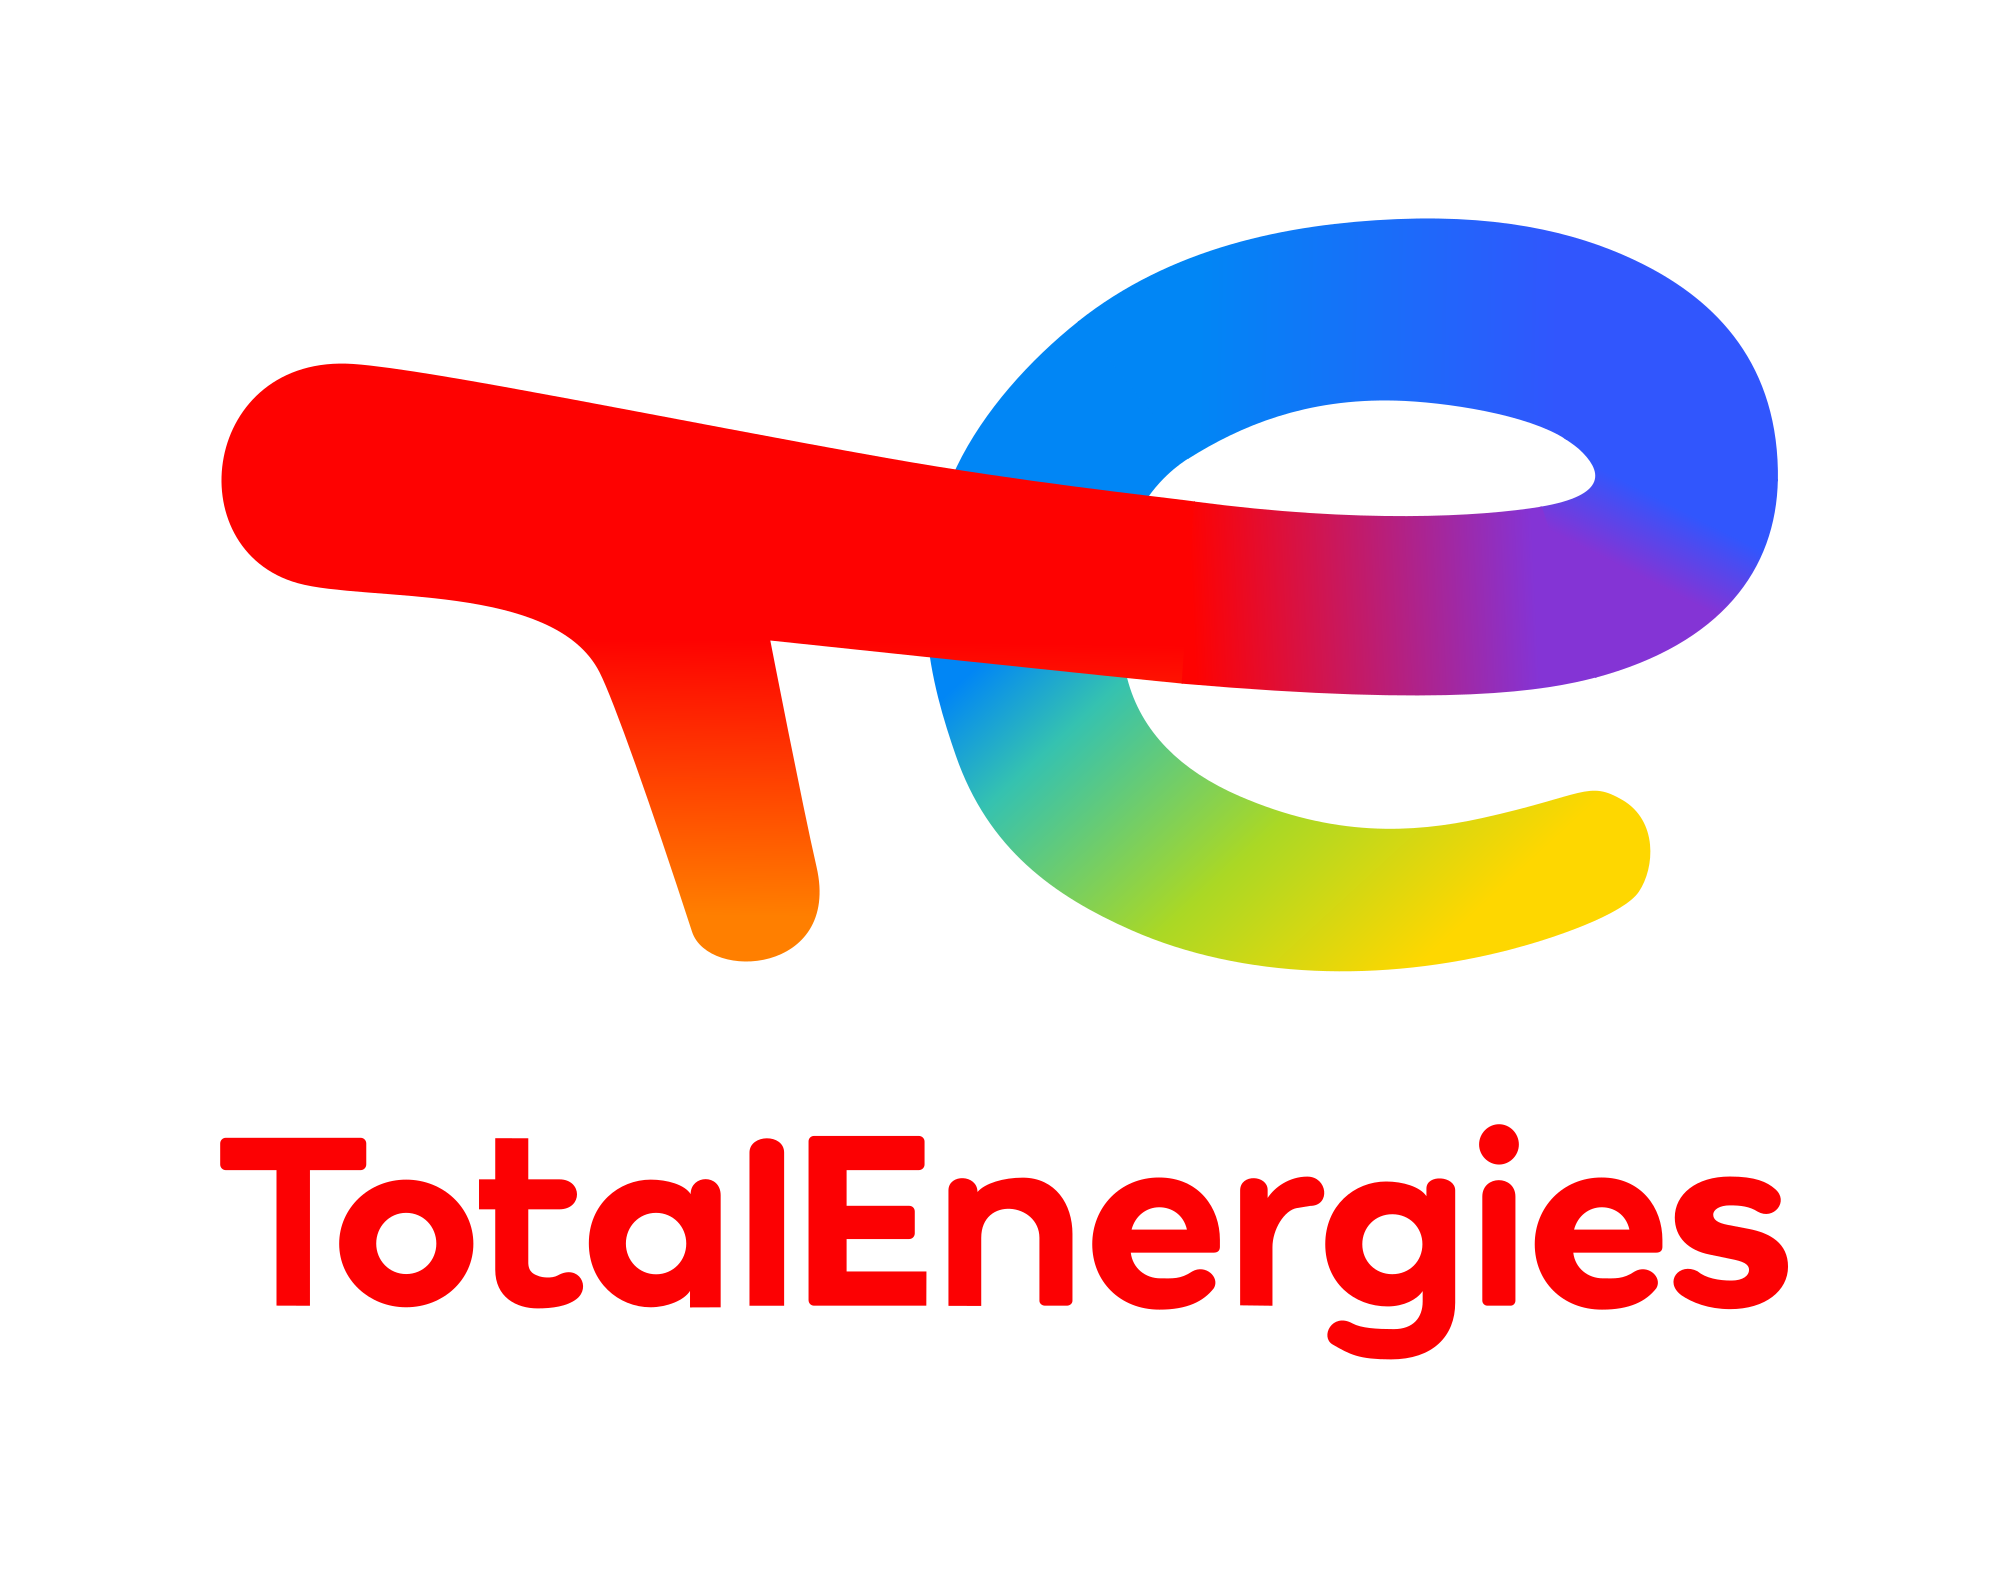
\includegraphics[width=0.25\textwidth]{total.png}\par\vspace{0.5cm}
    \vfill
    {\Large Bidan Marie, Mosse Joseph, Rubira Pierre\par}
    \vfill
    {\large Finance d'entreprise \par}
    {M1-MBFA-ARB - Année 2022-2023\par}

\end{titlepage}
\pagestyle{fancy}
\fancyhead{}
\fancyhead[R]{TotalEnergies}
\fancyhead[L]{\leftmark }
\fancyfoot{} 
\fancyfoot[R]{\thepage}


\section{Présentation du groupe TotalEnergies}
\subsection{L'histoire du groupe}
La compagnie a été créée le 28 mars 1924. C'est un acteur historique de l'énergie, elle a mis au jour de grands gisements dans le monde. Elle dispose d'un des plus grands réseaux de
production et de distribution. Tout au long de son existence, la compagnie a su diversifier ses activités et élargi ses implantations dans le monde. En se positionnant à ses débuts sur
les secteurs du gaz ou encore de la pétrochimie, jusqu'à amorcer une transition vers des énergies renouvelables comme le solaire ou encore les biocarburants. TotalEnergies est donc une
entreprise qui produit, transforme et transporte puis distribue. Elle fait figure de leader en 2021 sur ce secteur d'activité et compte parmi les entreprises pétrolières les plus
importantes au monde avec Shell, BP ou encore Saudi Aramaco. L'entreprise Total occupe toutes les activités sur le segment pétrolier et gazier. L'entreprise est à la fois productrice 
de gaz et de pétrole. Elle possède également des raffinerie et vend ses énergies transformées dans ses propres stations de carburant ainsi qu'à ses concurrents. Depuis plusieurs
décennies, Total diversifie également ses activités, et l'entreprise est de plus en plus engagée sur le marché des énergies renouvelables grâce à ses propres filiales comme Total Solar
qui est spécialisé dans les énergies solaires.

\subsection{Une multinationale}
TotalEnergies compte parmi ses rangs plus de 150 000 collaborateurs, la majorité travaillant sur le secteur Français. Impliquée dans plus de 140 pays, compte à travers le
monde plus de 17 000 stations d'essence. Cette multinationale regroupe près de 160 nationalités et plus de 740 métiers. 
\section{Analyse de la performance économique et financière}
\subsection{Analyse de l'activité et de la profitabilité de Total Energies}
Les indicateurs d'activité permettent de mesurer l'activité de l'entreprise, c'est-à-dire la fabrication d'un produit ou la mise à disposition d'un service ou d'une marchandise. Mesure 
effectuée à partir de la marge commerciale, de la production de l'exercice et de la valeur ajoutée.
Les entreprises créent de la richesse. D'un point de vue financier, la richesse créée se mesure avec un résultat. Pour avoir plus d'informations, le résultat de l'exercice obtenu dans
le compte de résultat (produits - charges) est décomposé. La profitabilité est la capacité d'une entreprise à générer un résultat par son activité. C'est le rapport entre un résultat
et des ventes.


Il faut néanmoins prendre des pincettes quand nous parlons de l'augmentation considérable des indices de profitabilités et de rentabilité du groupe TotalEnergies. En effet depuis la 
fin du confinement lié à la crise sanitaire de la Covid19, et de la disruption des chaines internationales, le prix des énergies est en augmentation. De ce 
fait, la performance de Total est en partie stimulée par l'augmentation du prix de vente de ses biens et services.
Prenons l'exemple du brent, celui-ci est passé de 44,2\$/b  au 4ème trimestre de 2020 à plus de 80\$/b au 4ème trimestre de 2021. Le prix à pratiquement doublé.
Pour sera faite en statique et dynamique (en $n-1$ et $n-2$), et l'entreprise sera comparée autres acteurs du secteur.

\subsubsection{Chiffre d'affaire}
Le chiffre d'affaire correspond à la somme des ventes de marchandises, produits fabriqués, des prestations de services et des produits des activités annexes
\begin{table}[H]
    \sffamily
    \centering
    \caption{Chiffre d'affaire}
    \label{table:CA}
    \begin{tabular}{l*{1}{rrrrrr}}
        \toprule
        \textit{(en millions de dollars)} & \textbf{2021} & 2020 & 2019 & Var $n-1$ & Var $n-2$ \\
        \midrule
        Total Energies & 205 863 & 140 685 & 200 316 & 46.33\% & 2.77\% \\
        \midrule
        BP & 157 739 & 105 944 & 159 307 & 48.89\% & -0.98\% \\
        Exxonmobil & 276 692 & 178 574 & 255 583 & 54.95\% & 8.26\% \\ 
        Shell & 261 504 & 180 543 & 344 877 & 44.84\% & -24.17\% \\
        Chevron & 155 606 & 94 471 & 139 865 & 64.71\% & 11.25\% \\ 
    \midrule
        Moyenne secteur & ~ & ~ & ~ & 51.94\% & -0.58\% \\
    \bottomrule
    \end{tabular}
\end{table}
On remarque une hausse de plus de 46\% du chiffre d'affaires entre 2021 et 2020. Cette augmentation peut être due à une augmentation des quantités vendues et deuxièmement à l'augmentation des prix. En 2020, le confinement a été un frein à la consommation et à la production ce qui peut expliquer cette forte baisse du chiffre d'affaires entre 2019 et 2020 du groupe. Néanmoins, il y a une augmentation du chiffre d'affaires en 2019 et 2021 preuve d'une évolution de l'activité.
Par rapport au secteur l'entreprise se trouve dans la moyenne, en ce qui concerne la reprise d'activité par rapport à 2020, mais semble relativement stagner par rapport a la variation par rapport à 2019.
\subsubsection{Bénéfice avant intérêts, impôts, dépréciations et amortissement}
Le BAIIA pour Total, aussi appelé \textit{EBITDA} (Earnings Before Interest, Tax, Depreciation and Amortization) similaire à l'EBE permet de jauger le degrés de création de richesse ainsi que la rentabilité de l'entreprise
\begin{table}[H]
    \sffamily
    \centering
    \caption{Bénéfice avant intérêts, impôts, dépréciations et amortissement}
    \label{table:EBITDA}
    \begin{tabular}{l*{1}{rrrrrr}}
    \toprule
        ~ & \textbf{2021} & 2020 & 2019 & Var $n-1$ & Var $n-2$ \\
        \cmidrule(r){1-1}\cmidrule(r){2-4}\cmidrule(r){5-6}
        TotalEnergies & 38 378	& 15 949	& 31 988 & 	140.63\% &	19.98\% \\
    \cmidrule(r){1-1}\cmidrule(r){2-4}\cmidrule(r){5-6}
    BP & 37 147 & 12 041 & 36 571 & 208.50\% &	1.58\% \\
    Exxonmobil & 52 761 & 12 797 & 36 229 & 312.29\% &	45.63\% \\
    Shell	& 55 004 &	26 915 &	60 148 &	104.36\% &	-8.55\% \\
    Chevron	& 40 825	& 14 289	& 36 322 & 	185.71\% &	-60.66\% \\
    \cmidrule(r){1-1}\cmidrule(r){2-4}\cmidrule(r){5-6}
        Moyenne secteur	&   ~      &        ~ &    ~	 &	190.30\%	&   -0.41\%  \\
    \bottomrule
    \end{tabular}
\end{table}
L'EBITDA de Total en 2021 est positif, l'entreprise est rentable. Par rapport aux années précédentes, le 
groupe à su augmenter sa production de richesse, en effet par rapport à 2020, elle plus que double son EBITDA pour
trouver un niveau supérieur à celui de 2019 soit une augmentation de 20\%. Ce résultat est d'autant plus  
satisfaisant, dans la mesure où les autres entreprises du secteur, n'ont pas su retrouver le même niveau de
rentabilité qu'elles avaient avant la crise sanitaire.
\subsubsection{Résultat opérationnel}
Le résultat opérationnel (\textit{EBIT}) exprime le résultat réalisé par l'entreprise à travers son exploitation. Ce 
solde intermédiaire ne prend pas en compte les éléments financiers de l'entreprise, ni les produits exceptionnels, ni les impôts. 
\begin{table}[H]
    \sffamily
    \centering
    \caption{Résultat opérationnel}
    \label{table:EBIT}
    \begin{tabular}{l*{1}{rrrrrr}}
    \toprule
        ~ & \textbf{2021} & 2020 & 2019 & Var $n-1$ & Var $n-2$ \\
    \cmidrule(r){1-1}\cmidrule(r){2-4}\cmidrule(r){5-6}
        TotalEnergies & 23 662	&-5 623	&16 213	&520.81\%	&45.94\% \\
    \cmidrule(r){1-1}\cmidrule(r){2-4}\cmidrule(r){5-6}
        BP & 13 008 & -22 000 & 7 680 & 159.13\% & 69.38\% \\ 
        Exxonmobil & 23 233 & -30 653 & 11 664 & 175.79\% & 99.19\% \\ 
        Shell & 27 828 & -25 741 & 24 747 & 208.11\% & 12.45\% \\ 
        Chevron & 15 860 & -5404 & 3 093 & 393.49\% & 412.77\% \\ 
    \cmidrule(r){1-1}\cmidrule(r){2-4}\cmidrule(r){5-6}
        Moyenne secteur & ~ & ~ & ~ & 291.46\% & 127.95\% \\ 
    \bottomrule
    \end{tabular}
\end{table}
En 2021, Total affiche un résultat opérationnel positif, l'exploitation elle même arrive donc à dégager un bénéfice.
C'est une bonne chose, si l'on compare a 2020, année durant laquelle le résultat fût négatif (a cause de la baisse 
d'activité liée au confinement), en effet le groupe à su revenir au delà de son résultat par rapport a 2019.
Comparé aux autres entreprises du secteur, la performance de Total est relativement similaire aux autres 
entreprises. Il est a noter que le résultat de 2021 pour toutes les entreprises est meilleur que celui de 2019, en 
raison d'une augmentation des coûts du pétrole en 2021. On peut calculer le taux de marge opérationnel de l'entreprise.
\begin{table}[H]
    \sffamily
    \centering
    \caption{Taux de marge opérationnelle}
    \label{table:marge_EBIT}
    \begin{tabular}{l*{1}{rrrrrr}}
    \toprule
        ~ & \textbf{2021} & 2020 & 2019 & Var $n-1$ & Var $n-2$ \\
    \cmidrule(r){1-1}\cmidrule(r){2-4}\cmidrule(r){5-6}
        TotalEnergies & 11.49\% 	& -4.00\%	& 8.09\%	&15.49\%	&3.40\% \\
    \bottomrule
    \end{tabular}
\end{table}
\subsubsection{Résultat net}
Le résultat net est le bénéfice (ou la perte d'une entreprise). Il est obtenu en faisant la différence entre tous les produits et charges d'une entreprise.
\begin{table}[H]
    \sffamily
    \centering
    \caption{Résultat net}
    \label{table:RE}
    \begin{tabular}{l*{1}{rrrrrr}}
    \toprule
        ~ & \textbf{2021} & 2020 & 2019 & Var $n-1$ & Var $n-2$ \\
    \cmidrule(r){1-1}\cmidrule(r){2-4}\cmidrule(r){5-6}
TotalEnergies & 16 366 & -7 336 & 11 438 & 323.09\% & 43.08\% \\ 
\cmidrule(r){1-1}\cmidrule(r){2-4}\cmidrule(r){5-6}
        BP & 8 487 & -20 729 & 4 190 & 140.94\% & 102.55\% \\ 
        Exxonmobil & 23 545 & -23 276 & 14 034 & 201.16\% & 67.77\% \\ 
        Shell & 20 630 & -21 534 & 16 432 & 195.80\% & 25.55\% \\ 
        Chevron & 15 689 & -5 561 & 2 848 & 382.13\% & 450.88\% \\ 
        \cmidrule(r){1-1}\cmidrule(r){2-4}\cmidrule(r){5-6}
        Moyenne secteur & ~ & ~ & ~ & 248.62\% & 137.97\% \\ 
    \bottomrule
\end{tabular}
\end{table}
Ici en 2021, le résultat de Total est positif, l'entreprise a réalisé un bénéfice de 16 366 millions
de dollars. Finalement il est a noter que ce résultat est assez similaire mécaniquement au résultat 
opérationnel.
\subsection{Analyse de la rentabilité}
\subsubsection{Rentabilité économique}
Le retour sur investissement moyen (ROACE) est un ratio financier qui calcule la rentabilité obtenue par rapport aux investissements qu'elle a fait.
\begin{table}[H]
    \sffamily
    \centering
    \caption{ROACE}
    \label{table:ROACE}
    \begin{tabular}{l*{1}{rrrr}}
    \toprule
        ~ & \textbf{2021} & 2020 & 2019 \\
    \cmidrule(r){1-1}\cmidrule(r){2-4}
        ROACE & 13.9\% 	& 4.00\%	& 9.8\% \\
    \bottomrule
    \end{tabular}
\end{table}
\subsubsection{Rentabilité financière}
Le ROE mesure la capacité des capitaux investis par les actionnaires et associés (capitaux propres) à 
dégager un certain niveau de profit.
\begin{table}[H]
    \sffamily
    \centering
    \caption{ROE}
    \label{table:ROE}
    \begin{tabular}{l*{1}{rrrr}}
    \toprule
        ~ & \textbf{2021} & 2020 & 2019 \\
    \cmidrule(r){1-1}\cmidrule(r){2-4}
        ROE & 16,9\% & 3,7\% & 10,4\% \\
    \bottomrule
    \end{tabular}
\end{table}
\subsubsection{Capacité d'autofinancement}
La capacité d'autofinancement (CAF) représente le flux potentiel de trésorerie dégagé par l'activité normale de 
l'entreprise. Ce flux de trésorerie est potentiel car il ne tient pas compte des décalages de trésorerie liés au 
cycle d'exploitation. Plus la valeur de la CAF est élevée, plus l'entreprise a des possibilités de : 
\begin{itemize}
    \item Distribuer des dividendes aux actionnaires
    \item Financer des investissements
    \item Rembourser des emprunts
\end{itemize}
La différence majeure entre la CAF et la MBA est donc que la MBA n'exclut pas l'impact des cessions sur le résultat
contrairement à la CAF. C'est pour cette raison que nous allons regarder la Marge Brute d'Autofinancement (MBA) et 
la Marge brute d'autofinancement hors frais financiers (DACF).
\begin{table}[H]
    \sffamily
    \centering
    \caption{MBA et CAF}
    \label{table:CAF}
    \begin{tabular}{l*{1}{rrrr}}
    \toprule
        ~ & \textbf{2021} & 2020 & 2019 \\
    \cmidrule(r){1-1}\cmidrule(r){2-4}
        MBA & 29 140 	& 15 697	& ~ \\
        CAF &  30 660         &   17 635        &   28 180     \\
    \bottomrule
    \end{tabular}
\end{table}
\section{Analyse de la solvabilité}
\subsection{Analyse de la structure financière}
Concernant la question de la solvabilité du groupe, nous obtenons un ratio de 
solvabilité de 0.3918 en 2021.
La ratio de solvabilité étant le rapport entre les capitaux propres sur le passif total du bilan 
consolidé du groupe, il est admit que le risque d'insolvabilité est faible lorsque le ratio de 
solvabilité est supérieur à 33\%. Cet indicateur nous montre que la question de la solvabilité de TotalEnergies n'est pas préoccupante.


De la même manière, les indicateurs d'autonomie financière (rapport entre les dettes financières et
les capitaux propres) et du niveau d'endettement (rapport entre le total des dettes et les capitaux 
propres), qui doivent être inférieur à 1, sont respectivement de 0.13 et de 0.826.
Cela témoigne également d'un faible risque d'insolvabilité.

Concernant l'analyse dynamique de la solvabilité, nous remarquons que les différents indicateurs de 
solvabilité sont relativement stables chaque année. Ainsi, en 2019 et même en 2020 où le contexte 
économique dû à la crise du Covid n'était pas positif pour le groupe TotalEnergies, le risque 
d'insolvabilité du groupe reste faible.
\begin{table}[H]
    \sffamily
    \centering
    \caption{Structure financière}
    \label{table:solva}
    \begin{tabular}{l*{1}{rrrr}}
    \toprule
~&\textbf{2021} & 2020 & 2019 \\ 
\cmidrule(r){1-1}\cmidrule(r){2-4}
Total passif & 293458 & 266132 & 273294 \\ 
Capitaux propres & 114999 & 106085 & 116778 \\ 
Dettes totales & 95102 & 64676 & 70244 \\ 
Dettes financières & 15035 & 17099 & 14819 \\ 
\cmidrule(r){1-1}\cmidrule(r){2-4}
Ratio de solvabilité & 0.39 & 0.40 & 0.43 \\ 
Autonomie financière & 0.13 & 0.16 & 0.13 \\ 
Niveau d'endettement & 0.83 & 0.61 & 0.60 \\ 
\bottomrule
\end{tabular}
\end{table}
\subsection{Analyse de la liquidité}
Concernant la question de la liquidité du groupe TotalEnergies, nous avons calculé 3 indicateurs 
différents permettant d'analyser la liquidité d'une entreprise ou d'un groupe.
Toutefois, seul le premier est normé, il s'agit de la liquidité générale (rapport entre l'actif à 
court-terme et le passif à court-terme) et il doit être supérieur à 1 pour que
la situation ne soit pas alarmante. Étant de 1.16 en 2021, nous en concluons que le groupe 
TotalEnergie ne souffre pas d'un problème de liquidité.

Les deux autres indicateurs ne sont pas normés, leur analyse n'est donc pertinente que si nous les 
comparons aux autres entreprises du secteur ou si nous adoptons un point de vue dynamique.
L'indicateur de liquidité restreinte (rapport  entre l'actif à court-terme sans les stock et le passif 
à court-terme), est plus élevé pour TotalEnergie (0.95) que pour Shell (0.79), mais plus bas 
que pour Chevron (1.02), mais en étant relativement proche.
L'indicateur de liquidité immédiate (rapport entre la trésorerie et le passif à court-terme) est plus 
élevé pour TotalEnergies (0.22) que pour Chevron (0.21) mais plus bas que pour Shell (0.39).
\begin{table}[H]
    \sffamily
    \centering
    \caption{Liquidité}
    \label{table:liquide}
    \begin{tabular}{l*{1}{rrrr}}
    \toprule
~&\textbf{2021} & 2020 & 2019 \\ 
\cmidrule(r){1-1}\cmidrule(r){2-4}
Actif à CT & 111136 & 79679 & 85265 \\ 
        Passif à CT & 95102 & 64676 & 70244 \\ 
        Stocks & 19952 & 14730 & 17132 \\ 
        Trésorerie & 21342 & 31268 & 27352 \\
\cmidrule(r){1-1}\cmidrule(r){2-4}
        Liquidité générale & 1.17 & 1.23 & 1.21 \\ 
        Liquidité restreinte & 0.96 & 1.00 & 0.97 \\ 
        Liquidité immédiate & 0.22 & 0.48 & 0.39 \\
\bottomrule
\end{tabular}
\end{table}
\section{Analyse des flux de trésorerie}
\subsection{Les flux de trésorerie d'exploitation}
Le tableau~\ref{table:fluxActivite} représente les flux de trésorerie d'exploitation, c'est-à-dire, les encaissements générés par les activités propres de l'entreprise comme la vente de biens et de services, et auxquels sont retirés les décaissements liés à l'exploitation.
\begin{table}[H]
    \sffamily
    \centering
    \caption{Flux de trésorerie d'exploitation}
    \label{table:fluxActivite}
    \begin{tabular}{l*{1}{rrrrrr}}
        \toprule
        ~ & \textbf{2021} & 2020 & 2019 & Var $n-1$ & Var $n-2$ \\
        \cmidrule(r){1-1}\cmidrule(r){2-4}\cmidrule(r){5-6}
        Total Energies & 30 410 & 14 803 & 24 685 & 105.43\% & 23.19\% \\ 
        \cmidrule(r){1-1}\cmidrule(r){2-4}\cmidrule(r){5-6}
        BP & 23 612 & 12 162 & 25 770 & 94.15\% & -8.37\% \\ 
        Exxonmobil & 48 129 & 14 668 & 29 716 & 228.12\% & 61.96\% \\ 
        Shell & 45 104 & 34 105 & 42 178 & 32.25\% & 6.94\% \\ 
        Chevron & 29 187 & 10 577 & 27 314 & 175.95\% & 6.86\% \\ 
        \cmidrule(r){1-1}\cmidrule(r){2-4}\cmidrule(r){5-6}
        Moyenne secteur & ~ & ~ & ~ & 127.18\% & 18.12\% \\
    \bottomrule
    \end{tabular}
\end{table}
Ici, pour les trois années, les flux sont positifs. Cela signifie que l'entreprise arrive à générer plus de fonds que ce qu'elle n'en dépense. Elle se sert par exemple de cet excédent pour verser des dividendes aux actionnaires. Outre une augmentation de plus de $100\%$ en 2021 par rapport à 2020 (année ayant généré de moindres flux en raison de la crise sanitaire), on remarque que l'entreprise arrive à dégager $+23,19\%$ de trésorerie due à son exploitation par rapport à l'année 2019. Ainsi, Total se démarque par rapport à d'autres entreprises du secteur, n'ayant pas réussi à générer autant de trésorerie en plus par rapport à 2019.
\subsection{Les flux de trésorerie d'investissement}
Dans le tableau~\ref{table:fluxInvest} sont représentés les flux de trésoreries d'investissement de Total, ainsi que ceux d'autres entreprises du secteur. Ce flux sera impacté négativement par les  investissements de l'entreprise (immobilisations, acquisitions de sociétés ou de titres, etc.). Au contraire, il sera impacté positivement par les désinvestissements de l'entreprise (cession d'actifs, titres etc.).
\begin{table}[H]
    \centering
    \sffamily
    \caption{Flux de trésorerie d'investissement}
    \label{table:fluxInvest}
    \begin{tabular}{l*{1}{cccccc}}
    \toprule
        ~ & \textbf{2021} & 2020 & 2019 & Var $n-1$ & Var $n-2$ \\ 
        \cmidrule(r){1-1}\cmidrule(r){2-4}\cmidrule(r){5-6}
        Total Energies & -13 656 & -13 079 & -17 177 & -4.41\% & 20.50\% \\
        \cmidrule(r){1-1}\cmidrule(r){2-4}\cmidrule(r){5-6}
        BP & -18079 & 3 956 & -8 817 & -557.00\% & -105.05\% \\ 
        Exxonmobil & -10 235 & -18 459 & -23 084 & 44.55\% & 55.66\% \\ 
        Shell & -4 761 & -13 278 & -15 779 & 64.14\% & 69.83\% \\ 
        Chevron & -5 865 & -6 965 & -11 458 & 15.79\% & 48.81\% \\
        \cmidrule(r){1-1}\cmidrule(r){2-4}\cmidrule(r){5-6}
        Moyenne secteur & ~ & ~ & ~ & -87.38\% & 17.95\% \\
    \bottomrule
    \end{tabular}
\end{table}
En 2021, pour Total, le flux est négatif, cela veut dire que l'entreprise investit plus que ce qu'elle ne désinvestit, en effet en 2021 elle aura investi 16 589 millions et désinvesti 2 933 millions. Cela semble être une bonne chose pour le long terme, la politique d'investissement de Total étant de consacrer 50\% de ses investissements au maintien de ses activités historiques (pétrole) et 50\% dans la croissance de ses exploitation de gaz, électricité et énergies renouvelables, afin d'atteindre la neutralité carbone.
Par rapport à 2020, l'entreprise a légèrement fait diminuer ce flux (-4.41\%), car elle à davantage investi, si l'on compare cette évolution aux autres entreprises du secteur, Total se démarque de la majorité qui ont pour leur part vu ce flux augmenter entre 2020 et 2021, signe de désinvestissements plus importants du côté de ses entreprises.
Par rapport à 2019, le flux d'investissement a augmenté (+20.50\%), 2019 ayant été marquée par le rachat d'actifs de Anadarko en Afrique (pour 3900 M). Mis à part ce rachat, les investissements corporels et incorporels n'ont fait qu' augmenter entre 2019 et 2021 (donc diminuer le flux d'investissement)
\subsection{Les flux de trésorerie de financement}
Les flux de trésorerie de financement représentent les flux nets de trésorerie employés pour
financer l'entreprise, (versement de dividendes, apport en capital, montants prêtés par les
actionnaires, emprunts émis et remboursés). Ils apportent une vision de la solidité financière d'une entreprise. 
\begin{table}[H]
    \centering
    \sffamily
    \caption{Flux de trésorerie de financement}
    \label{table:fluxFin}
    \begin{tabular}{l*{1}{cccccc}}
        \toprule
        ~ & \textbf{2021} & 2020 & 2019 & Var $n-1$ & Var $n-2$ \\ 
        \cmidrule(r){1-1}\cmidrule(r){2-4}\cmidrule(r){5-6}
Total Energies & -25497 & 1398 & -7709 & -1923.82\% & -230.74\% \\ 
\cmidrule(r){1-1}\cmidrule(r){2-4}\cmidrule(r){5-6}
BP & -18 079 & 3 956 & -8 817 & -557.00\% & -105.05\% \\ 
Exxonmobil & -35 423 & 5 285 & -6 618 & -770.26\% & -435.25\% \\ 
Shell & -34 664 & -7 224 & -35 209 & -379.84\% & 1.55\% \\ 
Chevron & -23 113 & -3 736 & -19 758 & -518.66\% & -16.98\% \\ 
\cmidrule(r){1-1}\cmidrule(r){2-4}\cmidrule(r){5-6}
Moyenne secteur & ~ & ~ & ~ & -829.92\% & -157.30\% \\ 
\bottomrule
    \end{tabular}
\end{table}
Pour l'année 2021, les flux de financement sont négatifs, cela veut donc dire que l'entreprise
rembourse des dettes ou verse des dividendes, plus qu'elle ne souscrit a des emprunts.
En effet en 2020, les flux de financement sont positifs pour le groupe car ce dernier a émis
un emprunt conséquent. Par rapport a 2019, ce flux a évolué négativement car l'entreprise 
rembourse les dettes contractées en 2020.
\section{Analyse des éléments extra-financiers}
\subsection{Analyse de la gouvernance de l'entreprise}
“Une gouvernance au service de notre ambition”.
La gouvernance est la manière dont une entreprise est organisée, gérée et contrôlée. Chez TotalEnergies, elle s'articule autour du Conseil d'administration et de la Direction générale.

Le conseil d'administration détermine les orientations stratégiques de la société et veille au bon fonctionnement des organes internes de contrôle, ainsi qu'à la qualité de l'information fournie aux actionnaires et au marché. Elle s'appuie sur ses 4 comités : audit, gouvernance et éthique, rémunération, stratégie \& RSE.

La direction générale constitue l'instance de direction 
Le Comité exécutif de Total est désormais composé de :
\begin{itemize}
    \item Patrick Pouyanné, Président-directeur général
    \item Arnaud Breuillac, Directeur général Exploration-Production
    \item Helle Kristoffersen, Directrice générale Strategy-Innovation
    \item Bernard Pinatel, Directeur général Raffinage-Chimie
    \item Philippe Sauquet, Directeur général Gas, Renewables \& Power
    \item Jean-Pierre Sbraire, Directeur Financier Groupe
    \item Namita Shah, Directrice générale People \& Social Responsibility
    \item Alexis Vovk, Directeur général Marketing \& Services
\end{itemize}
\subsection{Analyse de la politique RSE}
Total devient en 2021 TotalEnergies et se transforme en une compagnie multi-énergies avec pour ambition d'être 
un acteur majeur de la transition énergétique. TotalEnergies est une compagnie de production et de fourniture
d'énergies, comme le pétrole, le gaz et l'électricité. Sa principale ambition est de devenir un acteur majeur 
de la transition énergétique. Cela passe même par un nouveau logo représentant un spectre de couleurs,
symbolisant toutes les énergies. On constate donc une transformation du mode de production de l'énergie, par 
exemple la production d'énergie par des produits pétrolier passera de 55\% en 2019 à  35\% 2030. Total compte 
se lancer dans la production d'électricité par la méthode des biocarburant afin de réduire ses émissions de 
gaz à effet de serre. En 2015 le groupe a émis 46 MtCO2 et compte émettre entre 25-30 MtCO2 en 2030 pour finir 
à 0 émission en 2050. On pourra donc s'attendre à retrouver dans le bilan consolidé une augmentation du côté 
des investissements car le groupe TotalEnergies souhaite remplacer ses méthodes de production par des méthodes 
moins polluantes. 
Le budget en R\&D du groupe s'élève à 849 Millions \$ en 2021, avec la construction de 18 centres de R\&D dans 
le monde. Son principal objectif comme précédemment dit, est d'être un acteur majeur de la transition 
énergétique et d'atteindre la neutralité carbone d'ici l'horizon 2050. Tout d'abord en agissant sur la 
production d'énergie fortement carbonée, et en soutenant ses clients au travers de la transition énergétique.

TotalEnergies est composé 35,8\% de femmes et 64,2\% d'hommes, à noter que la part de femme dans l'entreprise 
est en constante augmentation notamment au sein des dirigeant. 23\% des dirigeants étaient des femmes en 2019 
contre 26,5\% en 2021. Le groupe s'appuie sur des valeurs et des principes qui s'engagent à respecter les droits humains. Il y a un effort effectué sur la sécurité des employés, qui se traduit par une 
baisse du taux de fréquence des accidents déclarés, de 0,81 en 2019 à 0,73 en 2021.
D'autre part la multinationale cherche à promouvoir un cadre de travail agréable et serein qui permet de 
motiver le développement de la production et donc des innovations. 

\subsection{Analyse de la politique d'investissement} 
Le groupe souhaite continuer sa stratégie de transformation en une compagnie multi-énergies pour se diriger 
vers une neutralité carbone. Par exemple en 2021 TotalEnergies à réduit considérablement ses investissements 
dans le secteur de la raffinerie et de la chimie par rapport à 2019 (avant Covid19). Une baisse 
de 7,02\%, de 1382 à 1285 millions de dollars.
Un investissement dans les énergies renouvelables en 2019 de 2 259 M\$ à 3 341 M\$ en 2021 soit une augmentation de 47,9\%.
En complément de ces nouveaux choix d'investissements, la multinationale met en oeuvre des programmes en R\&D visant cinq points : 
\begin{itemize}
    \item “power” qui couvre les énergies renouvelables 
    \item “CO2 sustainability” pour développer des technologies visant des solutions plus durables, des  
        technologies à faible empreinte carbone.
    \item “Upstream” vise à améliorer l'efficacité opérationnelle des activités d'explorations - production afin 
        de réduire les émissions de gaz à effet de serre et d'améliorer la gestion de l'eau et des sols.
    \item “Downstream Processes \& Polymers” participe aux recherches sur le recyclage des poly-mères et le   
        développement des biocarburants.
    \item “Fuels \& Lubricants” pour accompagner la transformation du monde des transports et les nouvelles 
        mobilités.
\end{itemize}
Pour citer quelques chiffres: 
La capacité brute de génération d'électricité renouvelable été de 43 GW en 2021 contre 28,6 GW en 2020 ce qui représente une augmentation de +50\%. De plus, nous pouvons ajouter que la production d'électricité à partir de sources renouvelables était de 6,8% en 2021 contre 4% en 2020 soit une variation de +71%.
Ce qui démontre bien l'ambition d'une décarbonisation de son activité.

De ce fait, les productions des raffineries ont nettement diminué, passant d'une production de 1606kb/j en 2019, à 1208 kb/j en 2020 et 1137 kb/j en 2021. Ce qui démontre une fois encore l'ambition du groupe de produire une énergie à faible empreinte carbone.




\end{document}